\input ../talk-header.tex
\title
{Machine Learning}
\subtitle{Notes from yesterdays}

% If you wish to uncover everything in a step-wise fashion, uncomment
% the following command: 
%\beamerdefaultoverlayspecification{<+->}

\begin{document}

\begin{frame}
  \titlepage
\end{frame}

\begin{frame}
  \frametitle{What is Machine Learning?}
  Learning is what we do when we can't explain how.
  \begin{itemize}
  \item Supervised
  \item Unsupervised
  \item Reinforcement
  \end{itemize}
\end{frame}

\begin{frame}
  \frametitle{Lots of maths}
  We'll try to ignore it, but it's there\dots
  \begin{itemize}
  \item Vector spaces and linear algebra
  \item Probability
  \item Statistics
  \item Optimisation theory
  \item Differential calculus
  \end{itemize}
  The curse of dimensionality.
\end{frame}

\begin{frame}
  \frametitle{Data Science}
  \begin{enumerate}
  \item Define the question of interest
  \item Get the data
  \item Clean the data
  \item Explore the data
  \item Fit statistical models
  \item Communicate the results
  \item Make your analysis reproducible
  \end{enumerate}
\end{frame}

\begin{frame}
  \frametitle{Data}
  \only<1>{\vphrase{Observational vs experimental}}
  \only<2>{\vphrase{Anecdote: it doesn't accumulate to be data.}}
  \only<3>{\cimgh{bias-variance.png}}
  \only<4>{\vphrase{Features}}
  \only<5>{\vphrase{Feature Engineering}}
  \only<6>{\vphrase{One of $K$ = one-hot encoding}}
  \only<7>{\vphrase{Outliers: don't ignore them!}}
\end{frame}

\begin{frame}
  \frametitle{Feature Engineering}
  \begin{enumerate}
  \item Brainstorm
  \item Pick some
  \item Make them
  \item Evaluate
  \item Repeat
  \end{enumerate}
\end{frame}

\begin{frame}
  \frametitle{Easy Features}
  \only<1>{\phrase{Text}\vspace{1cm}
    \centerline{bag of words}}
  \only<2>{\phrase{Images}\vspace{1cm}
    \centerline{corners, edges, point matching}}
  \only<3>{\vphrase{We'll see more}}
\end{frame}

\begin{frame}
  \frametitle{Linear Regression}
  \only<1>{
    \textbf{Problem:}  $\{(x_i, y_i)\}$.

    Given $x$, predict $\hat y$.

    Here $y$ is continuous.
  }

  \only<2>{ $x$: \textbf{explanatory} or \textbf{predictor} variable.

    $y$: \textbf{response} variable.

    \vspace{1cm}
    \purple{For some reason, we believe a linear model is a good idea.}
  }
  

\end{frame}

\begin{frame}
  \frametitle{Residuals}
  What's left over.
  \only<1>{
    \vspace{1cm}
    \begin{displaymath}
      \text{data} = \text{fit} + \text{residual}      
    \end{displaymath}
  }
  \only<2>{
    \vspace{1cm}
    \begin{displaymath}
      y_i = \hat y_i + e_i
    \end{displaymath}
  }
  \only<3>{
    Goal: small residuals.

    \vspace{1cm}
    \begin{displaymath}
      \sum e_i^2
    \end{displaymath}
  }
\end{frame}

\begin{frame}
  \frametitle{Logistic regression}
  \only<1>{\begin{bphrase}
      \begin{itemize}
      \item Binary output
      \item Classification
      \end{itemize}
    \end{bphrase}
  }
  \only<2>{\begin{itemize}
    \item Have: continuous and discrete inputs
    \item Want: class (0 or 1)
    \end{itemize}
  }
  \only<3>{Logistic (sigmoid, logit) function
    \begin{mphrase}
      g(z) = \frac{1}{1+e^{-z}}
    \end{mphrase}
  }
\end{frame}

\begin{frame}
  \frametitle{One vs Rest, One vs One}
  \only<1>{
    What I described yesterday:
    \begin{itemize}
    \item OvR (OvA): compute $k$ classifiers
    \item OvO: compute $k(k-1)/2$ classifiers
    \end{itemize}

    The missing point: the classifiers give scores, not just in/out answers.
  }
  \only<2>{
    One vs Rest:

    Accept the judgement of the classifier with the highest score.
  }
  \only<3>{
    One vs One:

    Classifiers vote.  Accept the class that gets the most votes.
  }
  \only<3>{
    Advantage:  Reduces multi-class classification to single-class classification.

    Disadvantage:  Classifier scores aren't necessarily comparable.  For example, classes
    may have very different numbers of members.
  }
\end{frame}

\begin{frame}
  \frametitle{Hyperparameters}
  \only<1>{
    \begin{itemize}
    \item The word hyperparameter is not well-defined.
    \item In most contexts, it is the parameters of the underlying distribution
    \item In training, we learn the parameters of the model
    \item We choose the hyperparameters to govern the training
    \item So we may want to experiment to learn the distribution
      parameters that best optimise our learned model's performance
    \end{itemize}
  }
\end{frame}

\begin{frame}
  \frametitle{Testing}
  \begin{itemize}
  \item Set aside (partition) data for testing (e.g., 70\% / 30\%)
  \item Learn on training set, test on testing set
  \item When searching hyperparameters, set aside again (e.g., 60\% / 20\% / 20\%)
  \end{itemize}
\end{frame}

\begin{frame}
  \frametitle{SVM}
  \cimghh{WuxyO.png}
\end{frame}

\begin{frame}
  \frametitle{Decision Trees}
  \only<1>{
    % https://www.pexels.com/photo/blue-geeen-and-orange-parrot-37833/
    % https://static.pexels.com/photos/37833/rainbow-lorikeet-parrots-australia-rainbow-37833.jpeg
    % CC0 license
    \vspace{-2cm}
    \cimgwb{rainbow-lorikeet-parrots-australia-rainbow.jpg}
  }
  \only<2>{\centerline{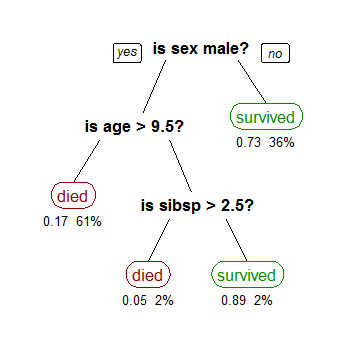
\includegraphics[height=.9\textheight]{tree_titanic_survivors.png}}
    % https://commons.wikimedia.org/wiki/File:CART_tree_titanic_survivors.png
    % License: CC ASA 3.0 unported.

    \vspace{-28mm}\parbox{.4\textwidth}{\red{E.g., passengers died
        with probability .17 which is 61\% of observations}}

    %\vspace{-18mm}
    \prevwork{Stephen Milborrow}
  }
  \only<3>{
    Variations
    \begin{itemize}
    \item Classification tree
    \item Regression tree
    \end{itemize}
  }
  \only<4>{
    % https://www.pexels.com/photo/nature-bird-australia-owl-105810/
    % https://static.pexels.com/photos/105810/pexels-photo-105810.jpeg
    % CC0 license
    \vspace{-3cm}
    \cimgwb{owl.jpg}
    \vspace{-8.7cm}
    \phrase{What can go wrong?}
  }
  \only<5>{
    Ensemble methods
    \begin{itemize}
    \item Bagging
    \item Random forest
    \item \gray{Boosted trees \textit{ (gradient boosted trees)}}
    \item \gray{Rotation forest}
    \end{itemize}
  }
\end{frame}

\begin{frame}
  \frametitle{Clustering}
  \cimgh{cluster-2.png}
\end{frame}

\begin{frame}
  \frametitle{Anomalies}
  Techniques:
  \begin{itemize}
  \item Density: kNN, local outlier factor
  \item SVM
  \item Clustering: $k$-Means
  \end{itemize}
\end{frame}

\begin{frame}
  \frametitle{NLP}
  \begin{itemize}
  \item Abstractive \ \ \gray{(hard)}
  \item Extractive \ \ \gray{(select sentences)}
  \end{itemize}
\end{frame}

%%%%%%%%%%%%%%%%%%%%%%%%%%%%%%%%%%%%%%%%%%%%%%%%%%%%%%%%%%%%%%%%%%%%%%
%\talksection{Break}

\begin{frame}
  % https://www.pexels.com/photo/landscape-mountains-nature-sky-45888/
  % https://static.pexels.com/photos/45888/landscape-scotland-nature-highlands-and-islands-45888.jpeg
  % CC0 license
  \cimgwb{skye-table.jpg}
  \vspace{-6.1cm}
  \phrase{questions?\hspace{2.2cm}}
\end{frame}

\end{document}
